% Copyright 2018 Melvin Eloy Irizarry-Gelpí
\setcounter{chapter}{11}
\chapter{Simple Harmonic Motion}
%%%%%%%%%%%%%%%%%%%%%%%%%%%%%%%%%%%%%%%%%%%%%%%%%%%%%%%%%%%%%%%%%%%%%%%%%%%%%%%%
...
%%%%%%%%%%%%%%%%%%%%%%%%%%%%%%%%%%%%%%%%%%%%%%%%%%%%%%%%%%%%%%%%%%%%%%%%%%%%%%%%
\section{Preliminary}
%%%%%%%%%%%%%%%%%%%%%%%%%%%%%%%%%%%%%%%%%%%%%%%%%%%%%%%%%%%%%%%%%%%%%%%%%%%%%%%%
When an elastic spring is stretched or compressed beyond its natural relaxed length, a restorative force arises on the spring that causes the spring to return to its natural relaxed length. This force is proportional to how much distance $x$ the spring is stretched:
\begin{equation} \label{eq.11.hooke}
    F_{k} = - k x
\end{equation}
Here the minus sign is due to the restorative nature of the force (it is always opposite to what the spring is doing), and $k$ is the spring constant.

If a mass $m$ is attached to one end of the spring, the mass will move back-and-forth when the spring is stretched or compressed. Due to Newton's second law, you have a relation between force and acceleration:
\begin{equation}
    F_{\text{net}} = m a \quad \Longrightarrow \quad -kx = m a
\end{equation}
Or in other words:
\begin{equation} \label{eq.11.ax}
    a = -\left( \frac{k}{m} \right) x
\end{equation}
That is, for this motion, the acceleration is proportional to the amount of distance that the spring is stretched or compressed. Note that the slope is negative.

When you look at the position as it change with time, it follows a pattern similar to a sine or cosine function, familiar from trigonometry. This suggest a sinusoidal fit for position $x$ as a function of time $t$:
\begin{equation}
    x(t) = A \sin{\left( Bt + C \right)} + D
\end{equation}
Here $A$ is the amplitude of the motion (in m), $B$ is the angular frequency (in rad/s), $C$ is the time shift (in rad), and $D$ is the position shift (in m). Velocity is defined as the rate of change of position with respect to time. With calculus, this is equivalent to taking a derivative with respect to time:
\begin{equation} \label{eq.11.v}
    v(t) = \frac{\mathrm{d} x}{\mathrm{d} t} = AB \cos{\left( Bt + C \right)}
\end{equation}
That is, the parameters that describe the fit for position ($A$, $B$, $C$, and $D$) can also be used to describe the fit for velocity. Similarly, acceleration is defined as the rate of change of velocity with respect to time. With calculus, this is equivalent to taking a derivative with respect to time:
\begin{equation} \label{eq.11.a}
    a(t) = \frac{\mathrm{d} v}{\mathrm{d} t} = -AB^{2} \sin{\left( Bt + C \right)}
\end{equation}
Again, the parameters that describe the fit for position can also be used to describe the fit for acceleration.

For a mass $m$ attached to a spring with spring constant $k$, the period of oscillation is given by
\begin{equation}
    T = 2\pi \sqrt{\frac{m}{k}}
\end{equation}
The period is the time it takes for the mass to do one full cycle. Related to the period is the angular frequency $\omega$:
\begin{equation} \label{eq.11.omega}
    \omega = \frac{2 \pi}{T} = \sqrt{\frac{k}{m}}
\end{equation}
As you are going to see, the same value of angular frequency controls how quickly position, velocity, acceleration, and force change with time.
%%%%%%%%%%%%%%%%%%%%%%%%%%%%%%%%%%%%%%%%%%%%%%%%%%%%%%%%%%%%%%%%%%%%%%%%%%%%%%%%
\section{Experiment}
%%%%%%%%%%%%%%%%%%%%%%%%%%%%%%%%%%%%%%%%%%%%%%%%%%%%%%%%%%%%%%%%%%%%%%%%%%%%%%%%
We are going to use a motion sensor to measure the position, velocity and acceleration of a mass hanging from a spring. The spring in turn hangs from a force sensor that we are going to use to measure force. When the sensor is zeroed correctly, the constant weight force $mg$ is taken into account. When the hanging mass is moved from equilibrium and released, the motion is oscillatory.

After recording data for a short time, you can use the LabQuest device to obtain the values of the parameters $A$, $B$, $C$, and $D$ that best describe the force and the position data versus time.

We are going to do four combinations of mass and spring constant, as stated in Table \ref{table.11.parameters}.
%%%%%%%%%%%%%%%%%%%%%%%%%%%%%%%%%%%%%%%%%%%%%%%%%%%%%%%%%%%%%%%%%%%%%%%%%%%%%%%%
\begin{table}
    \centering
    \begin{tabular}{|r|r|r|}\hline
        $k$ (N/m) & $m$ (kg) & $\omega$ (rad/s) \\ \hline
        5 & 0.05 & 10 \\
        5 & 0.1 & 7.071 \\
        15 & 0.1 & 12.247 \\
        15 & 0.15 & 10 \\
        \hline
    \end{tabular}
    \caption{Four combinations of mass and spring constant, along with $\omega$ prediction}
    \label{table.11.parameters}
\end{table}
%%%%%%%%%%%%%%%%%%%%%%%%%%%%%%%%%%%%%%%%%%%%%%%%%%%%%%%%%%%%%%%%%%%%%%%%%%%%%%%%
\section{Analysis}
%%%%%%%%%%%%%%%%%%%%%%%%%%%%%%%%%%%%%%%%%%%%%%%%%%%%%%%%%%%%%%%%%%%%%%%%%%%%%%%%
There are many aspects of simple harmonic motion that can be verified with this experiment.
%%%%%%%%%%%%%%%%%%%%%%%%%%%%%%%%%%%%%%%%%%%%%%%%%%%%%%%%%%%%%%%%%%%%%%%%%%%%%%%%
\subsection{Force and Position}
%%%%%%%%%%%%%%%%%%%%%%%%%%%%%%%%%%%%%%%%%%%%%%%%%%%%%%%%%%%%%%%%%%%%%%%%%%%%%%%%
You can verify Hooke's law, equation (\ref{eq.11.hooke}), by making a scatter plot chart with position in the horizontal axis, and force in the vertical axis. The shape of this graph is a downward line, as in Figure \ref{figure.11.hooke}. You can find the slope with the \texttt{SLOPE} function. If position is in column X with the first value in row 6, and force is in column Y, with first value in row 6; then the command is
\begin{center}
    \texttt{=SLOPE(Y6:Y, X6:X)}
\end{center}
The linear behavior confirms Hooke's law. The slope of the linear fit corresponds to the (negative) value of the spring constant. Conversely, the negative of the slope serves as an indirect measurement of the spring constant:
\begin{equation}
    k_{\text{exp}} = - (\text{slope of force versus position linear fit})
\end{equation}
Note that position and force data come from different sensors.
%%%%%%%%%%%%%%%%%%%%%%%%%%%%%%%%%%%%%%%%%%%%%%%%%%%%%%%%%%%%%%%%%%%%%%%%%%%%%%%%
\begin{figure}
    \centering
    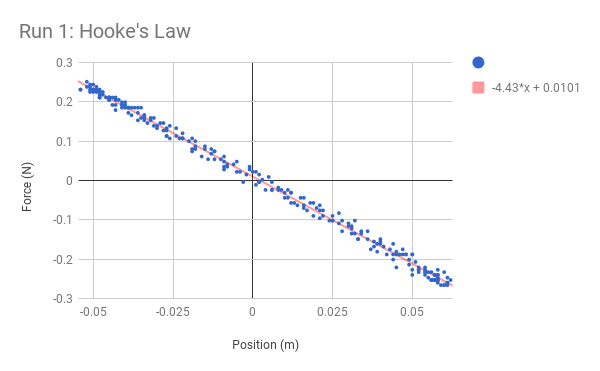
\includegraphics[scale=0.71]{image/11-shm/hooke.png}
    \caption{}
    \label{figure.11.hooke}
\end{figure}
%%%%%%%%%%%%%%%%%%%%%%%%%%%%%%%%%%%%%%%%%%%%%%%%%%%%%%%%%%%%%%%%%%%%%%%%%%%%%%%%
\subsection{Force and Acceleration}
%%%%%%%%%%%%%%%%%%%%%%%%%%%%%%%%%%%%%%%%%%%%%%%%%%%%%%%%%%%%%%%%%%%%%%%%%%%%%%%%
You can verify Newton's second law of motion by making a scatter plot chart with acceleration in the horizontal axis, and force in the vertical axis. The shape of this graph is an upward line, as in Figure \ref{figure.11.newton}. You can find the slope with the \texttt{SLOPE} function. The linear behavior confirms Newton's second law, and the value of the slope is mass. You can use this slope as an indirect measurement of the amount of mass hanging from the spring:
\begin{equation}
    m_{\text{exp}} = \text{slope of force versus acceleration linear fit}
\end{equation}
Note that acceleration and force data come from different sensors.

Together with the measurement of the spring constant from the force versus position graph, you can compute an experimental estimate of the angular frequency via
\begin{equation}
    \omega_{1} = \sqrt{\frac{k_{\text{exp}}}{m_{\text{exp}}}}
\end{equation}
%%%%%%%%%%%%%%%%%%%%%%%%%%%%%%%%%%%%%%%%%%%%%%%%%%%%%%%%%%%%%%%%%%%%%%%%%%%%%%%%
\begin{figure}
    \centering
    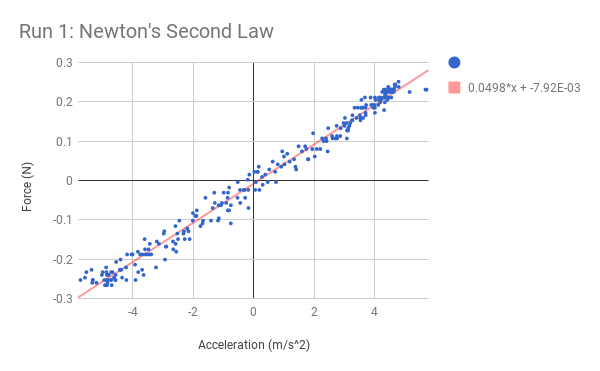
\includegraphics[scale=0.71]{image/11-shm/newton.png}
    \caption{}
    \label{figure.11.newton}
\end{figure}
%%%%%%%%%%%%%%%%%%%%%%%%%%%%%%%%%%%%%%%%%%%%%%%%%%%%%%%%%%%%%%%%%%%%%%%%%%%%%%%%
\subsection{Acceleration and Position}
%%%%%%%%%%%%%%%%%%%%%%%%%%%%%%%%%%%%%%%%%%%%%%%%%%%%%%%%%%%%%%%%%%%%%%%%%%%%%%%%
Combining Hooke's law with Newton's second law of motion gives equation (\ref{eq.11.ax}). Using the definition of $\omega$ in equation (\ref{eq.11.omega}), we find that indeed,
\begin{equation}
    a = -\omega^{2}x
\end{equation}
That is, for simple harmonic motion, the acceleration is proportional to the position with the slope being the (negative) squared angular frequency. The shape of this graph is a downward line, as in Figure \ref{figure.11.ax}. The slope of this graph is the negative of the squared angular frequency. This value provides another experimental estimate of the angular frequency:
\begin{equation}
    \omega_{2} = \sqrt{- (\text{slope of acceleration versus position})}
\end{equation}
%%%%%%%%%%%%%%%%%%%%%%%%%%%%%%%%%%%%%%%%%%%%%%%%%%%%%%%%%%%%%%%%%%%%%%%%%%%%%%%%
\begin{figure}
    \centering
    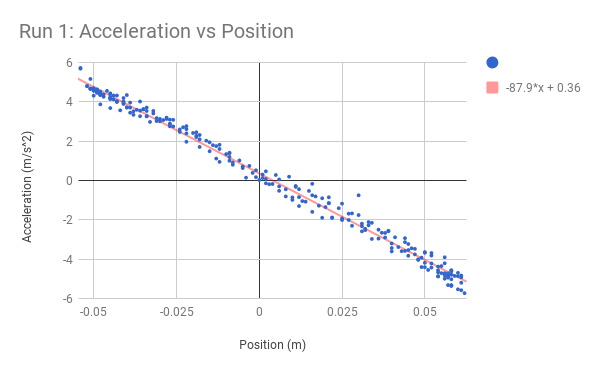
\includegraphics[scale=0.71]{image/11-shm/a-vs-x.png}
    \caption{}
    \label{figure.11.ax}
\end{figure}
%%%%%%%%%%%%%%%%%%%%%%%%%%%%%%%%%%%%%%%%%%%%%%%%%%%%%%%%%%%%%%%%%%%%%%%%%%%%%%%%
\subsection{Common Angular Frequency}
%%%%%%%%%%%%%%%%%%%%%%%%%%%%%%%%%%%%%%%%%%%%%%%%%%%%%%%%%%%%%%%%%%%%%%%%%%%%%%%%
From the LabQuest device, you can obtain the parameters for the sinusoidal fit for position and force. The values for $A$, $C$, and $D$ will not necessarily agree, but the values for $B$ in both fits should be very close. Indeed, the $B$ from the force and position fits provide yet more experimental estimates of the angular frequency:
\begin{equation}
    \omega_{3} = B \text{ from force fit}
\end{equation}
and
\begin{equation}
    \omega_{4} = B \text{ from position fit}
\end{equation}
Note that, since the data for position and force comes from different sensors, these measurements can be taken as fully independent.

In principle you can perform a sinusoidal fit on velocity and acceleration too. However, the parameters of these fits are not independent. Indeed, theoretically, they depend on the parameters for the position fit as stated in equations (\ref{eq.11.v}) and (\ref{eq.11.a}). In class we saw how you can use compute the fit functions in (\ref{eq.11.v}) and (\ref{eq.11.a}) with the parameters from the position fit, and how those function are in very good agreement with the experimental data collected.
%%%%%%%%%%%%%%%%%%%%%%%%%%%%%%%%%%%%%%%%%%%%%%%%%%%%%%%%%%%%%%%%%%%%%%%%%%%%%%%%
\subsection{Velocity and Position}
%%%%%%%%%%%%%%%%%%%%%%%%%%%%%%%%%%%%%%%%%%%%%%%%%%%%%%%%%%%%%%%%%%%%%%%%%%%%%%%%
A graph with velocity and position is called a phase space graph. For this particular experiment with simple harmonic motion, the velocity and position data yield an elliptical shape (a closed orbit), as in Figure \ref{figure.11.phase}. Now you know!
%%%%%%%%%%%%%%%%%%%%%%%%%%%%%%%%%%%%%%%%%%%%%%%%%%%%%%%%%%%%%%%%%%%%%%%%%%%%%%%%
\begin{figure}
    \centering
    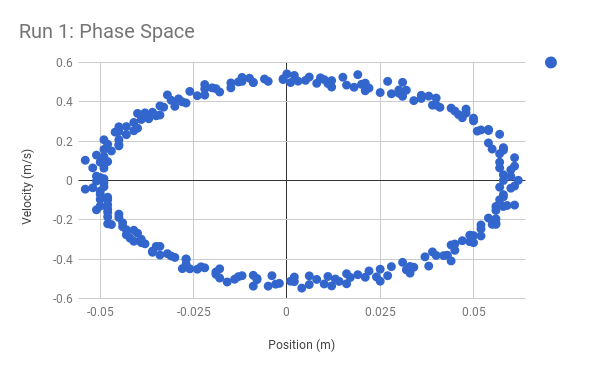
\includegraphics[scale=0.71]{image/11-shm/phase.png}
    \caption{}
    \label{figure.11.phase}
\end{figure}
%%%%%%%%%%%%%%%%%%%%%%%%%%%%%%%%%%%%%%%%%%%%%%%%%%%%%%%%%%%%%%%%%%%%%%%%%%%%%%%%
\section{My Data}
%%%%%%%%%%%%%%%%%%%%%%%%%%%%%%%%%%%%%%%%%%%%%%%%%%%%%%%%%%%%%%%%%%%%%%%%%%%%%%%%
The results for my run 1 are summarized in Table \ref{table.11.results}.
%%%%%%%%%%%%%%%%%%%%%%%%%%%%%%%%%%%%%%%%%%%%%%%%%%%%%%%%%%%%%%%%%%%%%%%%%%%%%%%%
\begin{table}
    \centering
    \begin{tabular}{|l|r|}
        \hline
        Name & Value \\
        \hline
        $m_{\text{exp}}$ & 0.0498 kg \\
        $k_{\text{exp}}$ & 4.4255 N/m \\
        $\omega_{1}$ & 9.4230 rad/s \\
        $\omega_{2}$ & 9.3776 rad/s \\
        $\omega_{3}$ & 9.5802 rad/s \\
        $\omega_{4}$ & 9.5796 rad/s \\
        \hline
        $\omega_{\text{ave}}$ & 9.4901 rad/s \\
        \hline
    \end{tabular}
    \caption{Results for run 1. The last row is the average of the previous four rows.}
    \label{table.11.results}
\end{table}
%%%%%%%%%%%%%%%%%%%%%%%%%%%%%%%%%%%%%%%%%%%%%%%%%%%%%%%%%%%%%%%%%%%%%%%%%%%%%%%%
\section{Your Data}
%%%%%%%%%%%%%%%%%%%%%%%%%%%%%%%%%%%%%%%%%%%%%%%%%%%%%%%%%%%%%%%%%%%%%%%%%%%%%%%%
...
%%%%%%%%%%%%%%%%%%%%%%%%%%%%%%%%%%%%%%%%%%%%%%%%%%%%%%%%%%%%%%%%%%%%%%%%%%%%%%%%
\newpage
\section{Your Laboratory Report}
%%%%%%%%%%%%%%%%%%%%%%%%%%%%%%%%%%%%%%%%%%%%%%%%%%%%%%%%%%%%%%%%%%%%%%%%%%%%%%%%
In your lab report you should include:
\begin{enumerate}
    \item A version of Table \ref{table.11.results} with four runs, one for each different mass/spring constant combination. You do not have to make the graphs in order to get the slopes; use the \texttt{SLOPE} function.
    \item One acceleration versus position graph with the linear fit, for a run of your choosing.
    \item One force versus acceleration graph with the linear fit, for a run of your choosing.
    \item One force versus position graph with the linear fit, for a run of your choosing.
    \item One velocity versus position graph for a run of your choosing.
\end{enumerate}
You should answer the following questions:
\begin{enumerate}
    \item Based on your analysis and what we saw in class, are you convinced that (for simple harmonic motion) all of position, velocity, acceleration, and force can be described by sines or cosines with a common angular frequency?
    \item Is the angular frequency parameter $B$ for the position versus time graph the same or close to the angular frequency parameter $B$ for the force versus time graph?
    \item Can you test Newton's second law with the data from this experiment? Does the measured mass agree with the expected value used?
    \item Can you test Hooke's law with the data from this experiment? Does the measured spring constant agree with the expected value used?
    \item Are your four estimates of the angular frequencies close to the expected theoretical value given by (\ref{eq.11.omega}).
\end{enumerate}
%%%%%%%%%%%%%%%%%%%%%%%%%%%%%%%%%%%%%%%%%%%%%%%%%%%%%%%%%%%%%%%%%%%%%%%%%%%%%%%%
\newpage
\section{Tables}
%%%%%%%%%%%%%%%%%%%%%%%%%%%%%%%%%%%%%%%%%%%%%%%%%%%%%%%%%%%%%%%%%%%%%%%%%%%%%%%%
\FloatBarrier
\newpage
\section{Figures}
%%%%%%%%%%%%%%%%%%%%%%%%%%%%%%%%%%%%%%%%%%%%%%%%%%%%%%%%%%%%%%%%%%%%%%%%%%%%%%%%
